\chapter{Cookie e Preferenze}\label{cap:cookie}

\begin{tcolorbox}[title=Mappa del capitolo]
Obiettivi, Impostazione/Lettura, Sicurezza, Esempi pratici, Caso di studio, Esercizi, Verifica, Riferimenti.
\end{tcolorbox}

\section{Obiettivi di apprendimento}
\begin{itemize}
  \item Configurare cookie con opzioni di sicurezza adeguate.
  \item Leggere, validare e serializzare valori cookie in sicurezza.
  \item Comprendere limiti e uso di SameSite/HttpOnly/Secure.
\end{itemize}

\section{Impostazione e lettura di un cookie}
Esempio di impostazione di un cookie con flag di sicurezza.

\begin{lstlisting}[language=PHP, caption={Cookie sicuri}]
<?php
$valore = json_encode(['tema' => 'scuro']);
setcookie('preferenze', $valore, [
  'expires' => time() + 3600*24*30,
  'path' => '/',
  'domain' => '',
  'secure' => true,
  'httponly' => true,
  'samesite' => 'Strict',
]);

echo htmlspecialchars($_COOKIE['preferenze'] ?? '');
?>
\end{lstlisting}

\subsection{Ciclo di vita dei Cookie}

I cookie seguono un ciclo preciso tra client (browser) e server:

\begin{center}
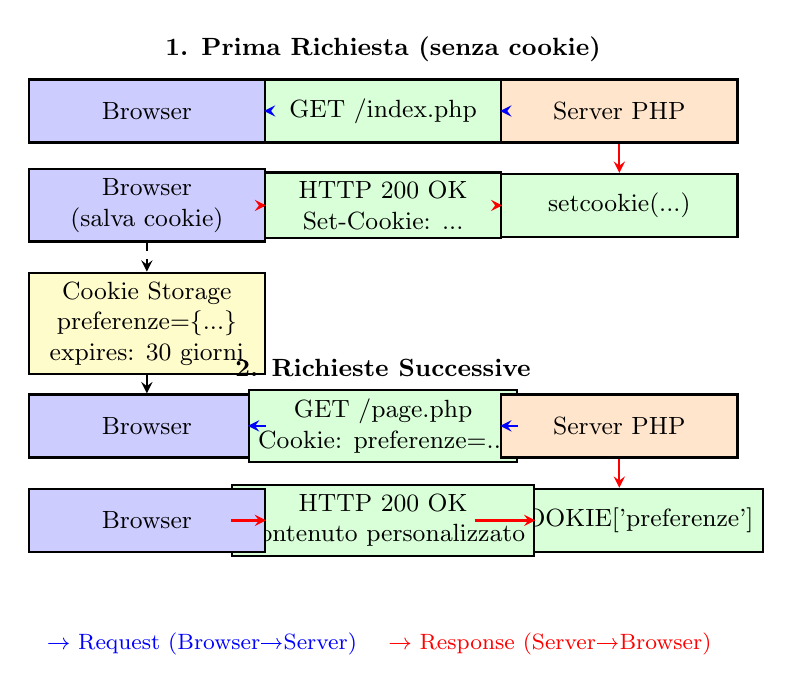
\begin{tikzpicture}[
    node distance=1.5cm,
    box/.style={rectangle, draw, thick, minimum width=3cm, minimum height=0.8cm, align=center, font=\small},
    client/.style={box, fill=blue!20},
    server/.style={box, fill=orange!20},
    action/.style={box, fill=green!15},
    arrow/.style={->, thick, >=stealth}
]
    % Prima richiesta
    \node[above, font=\small\bfseries] at (3,6.5) {1. Prima Richiesta (senza cookie)};

    \node[client] (browser1) at (0,6) {Browser};
    \node[action] (req1) at (3,6) {GET /index.php};
    \node[server] (server1) at (6,6) {Server PHP};

    \draw[arrow, blue] (browser1) -- (req1);
    \draw[arrow, blue] (req1) -- (server1);

    % Set-Cookie Response
    \node[action] (setcookie) at (6,4.8) {setcookie(...)};
    \node[action] (response1) at (3,4.8) {HTTP 200 OK\\Set-Cookie: ...};
    \node[client] (browser2) at (0,4.8) {Browser\\(salva cookie)};

    \draw[arrow, red] (server1) -- (setcookie);
    \draw[arrow, red] (setcookie) -- (response1);
    \draw[arrow, red] (response1) -- (browser2);

    % Storage
    \node[client, fill=yellow!20] (storage) at (0,3.3) {Cookie Storage\\preferenze=\{...\}\\expires: 30 giorni};

    \draw[arrow, dashed] (browser2) -- (storage);

    % Seconda richiesta
    \node[above, font=\small\bfseries] at (3,2.5) {2. Richieste Successive};

    \node[client] (browser3) at (0,2) {Browser};
    \node[action] (req2) at (3,2) {GET /page.php\\Cookie: preferenze=...};
    \node[server] (server2) at (6,2) {Server PHP};

    \draw[arrow] (storage) -- (browser3);
    \draw[arrow, blue] (browser3) -- (req2);
    \draw[arrow, blue] (req2) -- (server2);

    % Read Cookie
    \node[action] (readcookie) at (6,0.8) {\$\_COOKIE['preferenze']};
    \node[action] (response2) at (3,0.8) {HTTP 200 OK\\Contenuto personalizzato};
    \node[client] (browser4) at (0,0.8) {Browser};

    \draw[arrow, red] (server2) -- (readcookie);
    \draw[arrow, red] (readcookie) -- (response2);
    \draw[arrow, red] (response2) -- (browser4);

    % Legenda
    \node[below, font=\footnotesize, align=left] at (3,-0.5) {
        \textcolor{blue}{$\rightarrow$ Request (Browser→Server)} \quad
        \textcolor{red}{$\rightarrow$ Response (Server→Browser)}
    };
\end{tikzpicture}
\end{center}

\begin{tcolorbox}[colback=blue!10, colframe=blue!60, title=Punti chiave del ciclo di vita]
\begin{enumerate}
    \item \textbf{Prima richiesta}: Il browser richiede una pagina senza cookie
    \item \textbf{Set-Cookie}: Il server usa \texttt{setcookie()} per inviare un cookie nella risposta HTTP
    \item \textbf{Storage locale}: Il browser salva il cookie con le sue impostazioni (scadenza, path, domain, flags)
    \item \textbf{Richieste successive}: Il browser invia automaticamente il cookie in ogni richiesta che corrisponde a path/domain
    \item \textbf{Lettura server}: Il server legge il cookie da \texttt{\$\_COOKIE} e personalizza la risposta
\end{enumerate}
\end{tcolorbox}

\begin{attenzione}
I cookie sono \textbf{sempre inviati automaticamente} dal browser per ogni richiesta al dominio corrispondente. Questo rende necessari i flag di sicurezza:
\begin{itemize}
    \item \textbf{HttpOnly}: Previene accesso JavaScript (protezione XSS)
    \item \textbf{Secure}: Trasmissione solo su HTTPS (protezione man-in-the-middle)
    \item \textbf{SameSite}: Limita invio cross-site (protezione CSRF)
\end{itemize}
\end{attenzione}

\subsection{Analisi tecnica dei cookie sicuri}
\begin{itemize}
\item \textbf{Funzione e scopo}: Implementazione di cookie sicuri con protezioni complete contro attacchi XSS e session hijacking, utilizzando le opzioni di sicurezza disponibili in PHP.

\item \textbf{Componenti principali}:
\begin{itemize}
\item \texttt{json\_encode(['tema' => 'scuro'])}: Serializzazione dati strutturati per storage
\item \texttt{setcookie()} con array opzioni: Configurazione completa sicurezza
\item \texttt{expires}: Scadenza 30 giorni per cookie persistente
\item \texttt{path = '/'}: Accessibile in tutto il dominio
\item \texttt{secure = true}: Trasmissione solo HTTPS
\item \texttt{httponly = true}: Blocco accesso JavaScript
\item \texttt{samesite = 'Strict'}: Limitazione invii cross-site dei cookie
\item \texttt{htmlspecialchars(\$\_COOKIE[...] ?? '')}: Sanitizzazione output
\end{itemize}

\section{Caso di studio: preferenze tema e lingua}
Gestione di preferenze non sensibili (tema/lingua) tramite cookie JSON con opzioni \verb|httponly|, \verb|secure| e \verb|samesite| appropriate; validazione e fallback lato server in caso di valori assenti o corrotti.

\section{Esercizi}
\begin{itemize}
  \item Estendi l'esempio per includere la lingua preferita e valida i valori ammessi.
  \item Implementa una pagina che mostri le preferenze correnti con output opportunamente sanificato.
\end{itemize}

\section{Verifica}
\begin{itemize}
  \item Quali flag sono indispensabili per cookie di autenticazione?
  \item Quando \verb|SameSite=Strict| può causare problemi e quale alternativa usare?
\end{itemize}

\section{Riferimenti}
\begin{itemize}
  \item RFC 6265 — HTTP State Management Mechanism
  \item OWASP — Session Management
\end{itemize}

\item \textbf{Esempi pratici}: Questo pattern si applica in:
\begin{itemize}
\item Preferenze utente (tema, lingua, layout)
\item Token di autenticazione sicuri
\parametri di configurazione personalizzati
\item Carrelli acquisto e sessioni utente
\end{itemize}

\item \textbf{Varianti e alternative}:
\begin{itemize}
\item \texttt{setrawcookie()} per valori non URL-encoded
\item \texttt{session\_set\_cookie\_params()} per configurazione globale
\item Cookie cifrati con OpenSSL per dati sensibili
\item LocalStorage/SessionStorage per dati client-side
\item HttpOnly session cookies per autenticazione
\end{itemize}

\item \textbf{Best practices e insidie}:
\begin{itemize}
\item \textbf{Best practice}: Sempre \texttt{httponly} e \texttt{secure} per dati sensibili
\item \textbf{Insidia}: Cookie impostati dopo output HTML causano errori headers
\item \textbf{Sicurezza}: Validare e sanitizzare tutti i valori cookie
\item \textbf{Performance}: Limitare dimensione cookie (max 4KB)
\item \textbf{Compatibilità}: \texttt{samesite} supportato da Chrome/Firefox/Safari
\end{itemize}

\item \textbf{Riferimenti teorici}:
\begin{itemize}
\item \textbf{HTTP Cookies}: Standard RFC 6265 per gestione cookie
\item \textbf{SameSite Cookies}: Limitazione condivisione cross-site dei cookie
\item \textbf{Content Security Policy}: Difesa avanzata XSS
\item \textbf{JSON Serialization}: Formato dati strutturati per storage
\item \textbf{Secure Flag}: Enforcement HTTPS per trasmissione sicura
\end{itemize}
\end{itemize}
